\section{Text recognition model}
\label{subsec:ch5sec4}

\begin{figure}[htbp]
    \centering
        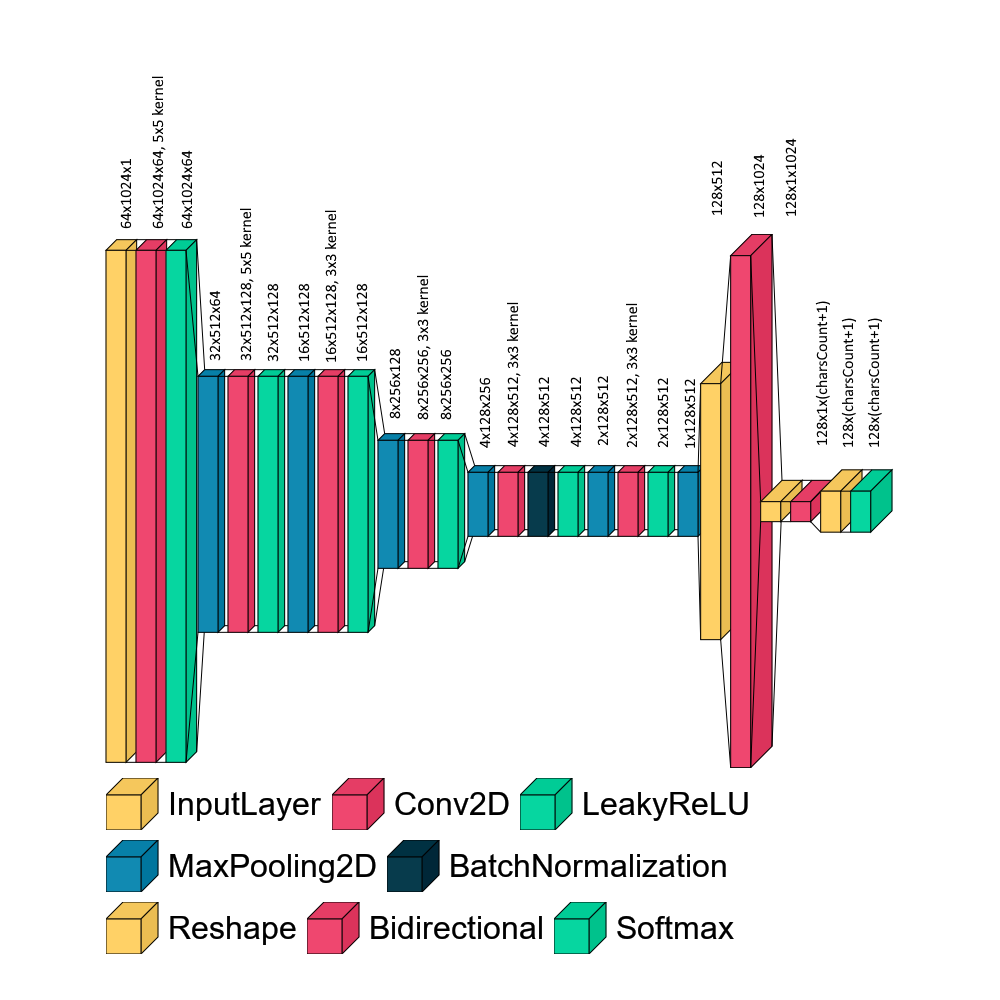
\includegraphics[scale=0.4]{figures/recog_model}
    \caption{Recognition model \cite{visualKeras}}
    \label{FigRecogModel}        
\end{figure}

Once the lines extraction is ready, each individual line can be preprocessed to a certain degree by slope correction, increasing contrast, enhancing strokes \cite{Juan} and then fed into the recognition model. The model input is a 1024px wide and 64px tall image. The segmented line is fit into these bounds by rescaling both dimensions by a factor. If the aspect ratio cannot be maintained (this happens when the line width is of a great length), squeezing is accepted unless the distortion is too high. In the less likely case of a line that cannot be fit into these bounds, splitting it horizontally would be a fine workaround.

A CNN-BiLSTM-CTC based architecture \cite{cnnbilstm} was selected for the recognition task --- see Figure \ref{FigRecogModel}.  The model consists of 6 convolution layers, the first two using a 5x5 kernel to enforce a wider feature extraction area. Pooling layers help to model the data into a vector of features. The last two of them take advantage of the wider width of the feature map \cite{cnnbilstm} and keep the height constant when it becomes of a small enough size. After the bidirectional LSTM later, another convolution layer with a wide kernel finally builds up the CTC values (see section \ref{subsec:ch3sec3subsec4subsubsec4}).

